\section{Auswertung}
\label{sec:Auswertung}
Bei diesem Versuch soll der Kernspin, die Landé-Faktoren und das Verhältnis von $\ce{^85Rb}$ und $\ce{^87Rb}$ ermittelt 
werden. Zusätzlich kann die Horizontalkomponente des Erdmagnetfelds bestimmt werden. Die dafür benötigten Daten sind in 
Tabelle \ref{tab:Messdaten_roh} aufgelistet.
\FloatBarrier
\begin{table}
  \centering
  \caption{Messdaten für die Bestimmung des Kernspins, die Landé-Faktoren und des Erdmagnetfelds.}
  \label{tab:Messdaten_roh}
  \begin{tabular}{c c c c c}
    \toprule
    &\multicolumn{2}{c}{Peak 1}&\multicolumn{2}{c}{Peak 2}\\
    \cmidrule(lr){2-3}\cmidrule(lr){4-5}
    Frequenz / $\SI{}{\kilo\hertz}$&Sweep&Horizontal&Sweep&Horizontal\\
    \midrule
    $\num{100}$&$\num{5.49}$ &$\num{13.8}$ &$\num{6.68}$&$\num{13.8}$\\
    $\num{200}$&$\num{6.01}$ &$\num{13.86}$&$\num{8.36}$&$\num{13.86}$\\
    $\num{300}$&$\num{5.43}$ &$\num{13.92}$&$\num{8.97}$&$\num{13.92}$\\
    $\num{400}$&$\num{3.79}$ &$\num{14.02}$&$\num{8.47}$&$\num{14.02}$\\
    $\num{500}$&$\num{2.64}$ &$\num{14.10}$&$\num{8.54}$&$\num{14.10}$\\
    $\num{600}$&$\num{1.86}$ &$\num{14.26}$&$\num{8.98}$&$\num{14.26}$\\
    $\num{700}$&$\num{1.37}$ &$\num{14.22}$&$\num{3.64}$&$\num{14.36}$\\
    $\num{800}$&$\num{3.76}$ &$\num{14.36}$&$\num{3.73}$&$\num{14.44}$\\
    $\num{900}$&$\num{2.55}$ &$\num{14.30}$&$\num{7.30}$&$\num{14.44}$\\
    $\num{1000}$&$\num{4.94}$&$\num{14.30}$&$\num{4.71}$&$\num{14.58}$\\
    \bottomrule
  \end{tabular}
\end{table} 
\FloatBarrier
Die Messdaten aus Tabelle \ref{tab:Messdaten_roh} müssen zunächst in eine Stromstärke umgerechnet werden. Die Sweepeinstellung 
muss mit dem Wert $\SI{0.1}{\ampere}$ und die Horizontaleinstellung mit $\SI{0.3}{\ampere}$ multipliziert werden um eine Stromstärke
zu erhalten. Bei der Horizontalkomponente ist ein Offset von $\num{13.8}$ vorhanden, daher muss dieser Wert von den Daten 
subtrahiert werden. Um aus den Stromstärken ein $B$-Wert zu erhalten muss die Formel 
\begin{equation*}
  B=\mu_0\frac{8\cdot N \cdot I}{\sqrt{125}R}
\end{equation*}
angewendet werden. Die Sweep- und Horizontalwerte müssen zum gesamt $B$-Wert addiert werden. Die Stromstärken und die 
$B$-Werte sind in Tabelle \ref{tab:Messdaten} zu sehen.
\begin{table}
  \centering
  \caption{Stromstärken und Magnetfeldstärke in abhängigkeit der Frequenz.}
  \label{tab:Messdaten}
  \begin{tabular}{c c c c c c c}
    \toprule
    &\multicolumn{3}{c}{Peak 1}&\multicolumn{3}{c}{Peak 2}\\
    \cmidrule(lr){2-4}\cmidrule(lr){5-7}
    $f\,/\,\SI{}{\kilo\hertz}$&$I_{\text{sweep}}\,/\,\SI{}{\ampere}$&$I_{\text{horizontal}}\,/\,\SI{}{\ampere}$&$B\,/\,\SI{}{\micro\tesla}$&$I_{\text{sweep}}\,/\,\SI{}{\ampere}$&$I_{\text{horizontal}}\,/\,\SI{}{\ampere}$&$B\,/\,\SI{}{\micro\tesla}$\\
    \midrule
    $\num{100}$ &$\num{0.549}$&$\num{0.0}$  &$\num{33.1}$&$\num{0.668}$&$\num{0.0}$&$\num{40.3}$\\
    $\num{200}$ &$\num{0.601}$&$\num{0.018}$&$\num{52.1}$&$\num{0.836}$&$\num{0.018}$&$\num{66.2}$\\
    $\num{300}$ &$\num{0.543}$&$\num{0.036}$&$\num{64.3}$&$\num{0.897}$&$\num{0.036}$&$\num{85.7}$\\
    $\num{400}$ &$\num{0.379}$&$\num{0.066}$&$\num{80.8}$&$\num{0.847}$&$\num{0.066}$&$\num{109.0}$\\
    $\num{500}$ &$\num{0.264}$&$\num{0.089}$&$\num{94.9}$&$\num{0.854}$&$\num{0.09}$&$\num{130.5}$\\
    $\num{600}$ &$\num{0.186}$&$\num{0.138}$&$\num{132.2}$&$\num{0.898}$&$\num{0.138}$&$\num{175.2}$\\
    $\num{700}$ &$\num{0.137}$&$\num{0.126}$&$\num{118.8}$&$\num{0.364}$&$\num{0.168}$&$\num{169.3}$\\
    $\num{800}$ &$\num{0.376}$&$\num{0.168}$&$\num{170.0}$&$\num{0.373}$&$\num{0.192}$&$\num{190.9}$\\
    $\num{900}$ &$\num{0.255}$&$\num{0.15}$ &$\num{146.9}$&$\num{0.73}$&$\num{0.192}$&$\num{212.4}$\\
    $\num{1000}$&$\num{0.494}$&$\num{0.15}$ &$\num{161.4}$&$\num{0.471}$&$\num{0.234}$&$\num{233.6}$\\
    \bottomrule
  \end{tabular}
\end{table}
\FloatBarrier
Die Magnetfeldstärke wird gegen die Frequenz aufgetragen und es wird eine lineare Ausgleichsgrade
\begin{equation*}
  \label{eq:lin_fit}
  f(B)=a\cdot B + b
\end{equation*}
bestimmt. 
Mithilfe der Aufspaltung des Zeemaneffekts kann der Landé-Faktor bestimmt werden.
\begin{gather*}
  \Delta E = hf = g_{\text{F}} \mu_{\text{B}} B\\
  \implies a = \frac{g_{\text{F}} \mu_{\text{B}}}{h} \\
  \implies g_{\text{F}} = \frac{h}{a\mu_{\text{B}}}
\end{gather*}
Der y-Achsenabschnitt $b$ kann mit dem Erdmagnetfeld gleichgesetzt werden. Die lineare Ausgleichsgrade ist zusammen mit 
den Messdaten in Abbildung \ref{fig:Fit_Messdaten} abgebildet.
\FloatBarrier
\begin{figure}
  \centering
  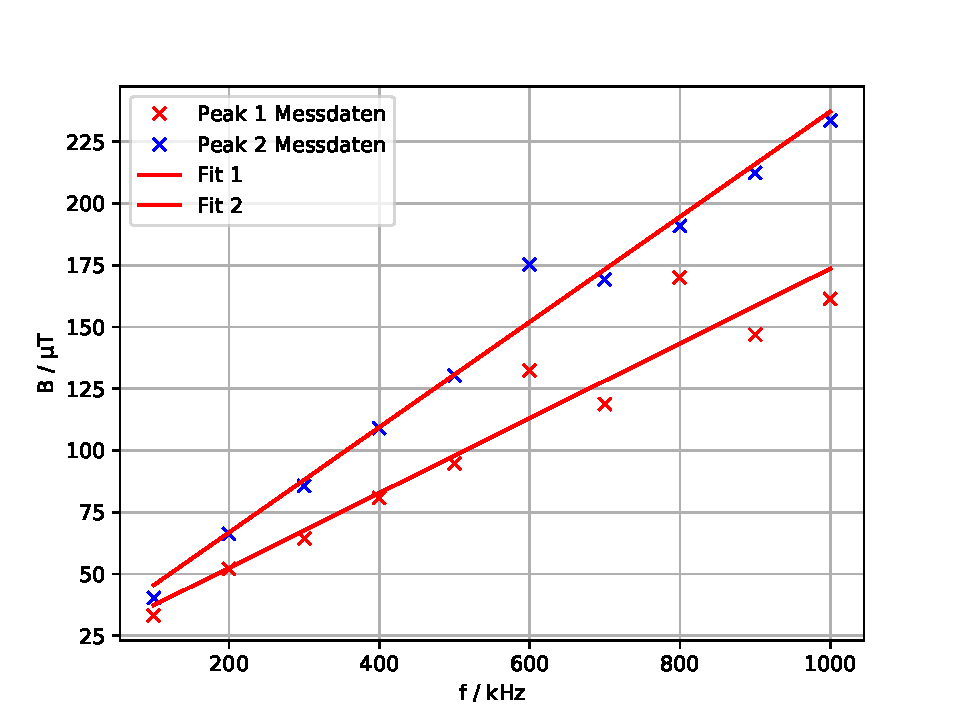
\includegraphics[width = \textwidth,keepaspectratio]{figure/Messdaten_Fit.pdf}
  \caption{Messdaten und Ausgleichsgrade für die Bestimmung der Landé-Faktoren und des Erdmagnetfelds.}
  \label{fig:Fit_Messdaten}
\end{figure}
\FloatBarrier
Die Fitparameter der Ausgleichsgraden aus Abbildung \ref{fig:Fit_Messdaten} sind in Tabelle \ref{tab:FitParams} aufgelistet.
\begin{table}
  \centering
  \caption{Fitparameter der beiden Ausgleichsgraden.}
  \label{tab:FitParams}
  \begin{tabular}{c c c}
    \toprule
    Peak&$a\,/\,\SI{}{\hertz\per\tesla}$&$b \,/\,\SI{}{\micro\tesla}$\\
    \midrule
    1&$\num{1.51(15)e-10}$&$\num{22(9)}$\\
    2&$\num{2.13(10)e-10}$&$\num{24(6)}$\\
    \bottomrule
  \end{tabular}
\end{table}
\FloatBarrier
Die Erdmagnetfeldstären können zu dem Wert $b=\SI{23(5)}{\micro\tesla}$ gemittelt werden. Der Theoriewert von $b_{\text{theo}}=\SI{20}{\micro\tesla}$
liegt in der Unsicherheit des experimentell bestimmten Werts. 
Die aus der Steigung bestimmten Landé-Faktoren betragen $g_{\text{F1}}=\num{0.47(5)}$ und $g_{\text{F2}} = \num{0.335(15)}$.
Um aus den Landé-Faktoren den Kernspin zu bestimmen wird die Gleichung \ref{karina_jan_gleichung_2} nach $I$ umgestellt.
\begin{equation*}
  I=J=\left(\frac{g_{\text{J}}}{g_{\text{F}}}-1\right)
\end{equation*}
Die bestimmten Werte betragen 
\begin{gather*}
  I_1 = \num{1.62(21)}\\
  I_2 = \num{2.48(14)}.
\end{gather*}
Die Theoriewerte sind $I_1 = \frac{3}{2}= \num{1.5}$ und $I_2 = \frac{5}{2}=\num{2.5}$, diese liegen innerhalb der Unsicherheiten der
experimentell bestimmten Werte.
\subsection{Isotopenverhältnis}
Um Das Isotopenverhältnis zu bestimmen werden die Amplituden der Peaks bei $f= \SI{100}{\kilo\hertz}$ bestimmt.
Dafür wird das Programm Inkscape \cite{??} verwendet. Die Amplituden aus Abbildung \ref{fig:Isotopenverhältnis} 
betragen $P_{1} = \SI{119.76}{px}$ und $P_{2} = \SI{221.94}{px}$. Das Verhältnis ist dann $\frac{P_2}{P_1} = \num{1.85}$.
Der Literaturwert beträgt $\frac{\num{72.168}}{\num{27.835}} = \num{2.59}$.
\FloatBarrier
\begin{figure}
  \centering
  \includegraphics[width = \textwidth,keepaspectratio]{figure/Oszibild.pdf}
  \caption{Typische Aufnahme bei $f=\SI{100}{\kilo\hertz}$, für die Bestimmung des Isotopenverhältnisses.}
  \label{fig:Isotopenverhältnis}
\end{figure}
